% !TEX program = xelatex
\documentclass[UTF8,a4paper,zihao=-4]{ctexart}

\usepackage[margin=2.2cm]{geometry}
\usepackage{amsmath,amssymb,bm}
\usepackage{graphicx}
\usepackage{booktabs}
\usepackage{tabularx}
\usepackage{longtable}
\usepackage{multirow}
\usepackage{siunitx}
\usepackage{caption}
\usepackage{subcaption}
\usepackage{float}
\usepackage{hyperref}
\usepackage{xcolor}
\usepackage{enumitem}
\usepackage{setspace}

\hypersetup{
  colorlinks=true,
  linkcolor=black,
  citecolor=black,
  urlcolor=blue!50!black
}

\graphicspath{{../results/}}
\sisetup{detect-all=true}

\title{\textbf{系泊系统的设计}}
\author{
  2016\,高教社杯全国大学生数学建模竞赛 A 题\\[0.4em]
  \small Freeze:~2016A-mooring-F2\quad
  主模型：离散多刚体静力（分段水平张力）+ Pareto 约束设计
}
\date{}

\begin{document}
\maketitle
\thispagestyle{empty}

\begin{abstract}
针对近浅海观测网传输节点的系泊系统设计，建立浮标--钢管--钢桶--重物球--锚链的平面静力模型。
锚链按无档链环节长离散（基线），并以连续悬链积分作对照；
水流作用下水平张力沿构件分段递推，链长强制为附表节长的整数倍。
在海水静止、水深 \SI{18}{m}、II 型链 \SI{22.05}{m}、球重 \SI{1200}{kg} 时：
风速 \SI{12}{m/s} 下钢桶倾角约 \(1.20^\circ\)、存在约 \SI{6.25}{m} 趴链，游动半径约 \SI{14.65}{m}；
\SI{24}{m/s} 下钢桶约 \(4.57^\circ\)、锚端夹角约 \(4.66^\circ\)；
\SI{36}{m/s} 下两约束均突破。
将球重调至 \textbf{\SI{2238}{kg}} 可使 \SI{36}{m/s} 时钢桶倾角 \(\le 5^\circ\) 且锚端夹角 \(\le 16^\circ\)。
综合风、流与 \(16\!-\!20\,\mathrm{m}\) 水深，在硬约束与软裕度下由 Pareto 前沿推荐
\textbf{IV 型链、长 \SI{28.05}{m}（187 节）、球重 \SI{5000}{kg}}；
训练、hold-out 及 252 点稠密扫描均满足硬约束。
局限：静水静力与平面假设，未计入波浪与三维流向；问题 3 为离散网格上的折中推荐而非连续全局唯一最优。

\vspace{0.6em}
\noindent\textbf{关键词：}系泊系统；静力平衡；分段水平张力；趴链；Pareto 设计
\end{abstract}

\tableofcontents
\newpage

\section{问题重述与答题清单}

系泊系统由浮标、4 节钢管、密封钢桶（含水声设备）、可选重物球、电焊锚链与抗拖移锚组成。
需在锚端切线与海床夹角 \(\le 16^\circ\)、并尽量控制钢桶倾角（超过 \(5^\circ\) 时设备效果较差）的前提下，
减小吃水与游动区域。

\begin{table}[H]
\centering
\caption{答题清单}
\begin{tabular}{clp{8.2cm}}
\toprule
子问 & 本文对应 & 交付内容 \\
\midrule
问题 1 & \S\ref{sec:q1} & 风速 \(12,24\,\mathrm{m/s}\) 的倾角、链形、吃水、游动半径 \\
问题 2 & \S\ref{sec:q2} & \(36\,\mathrm{m/s}\) 状态；调节球重使 \(\theta\le 5^\circ,\varphi\le 16^\circ\) \\
问题 3 & \S\ref{sec:q3} & 风+流+变水深下的型号/整数链长/球重方案与情景表 \\
\bottomrule
\end{tabular}
\end{table}

\section{问题分析与方案池}

各子问属静力机构求解与约束设计。按机制族给出三类方案：

\begin{table}[H]
\centering
\caption{跨机制族方案池}
\begin{tabular}{clp{7.5cm}}
\toprule
方案 & 机制族 & 角色 \\
\midrule
A & 离散多刚体铰接静力 + 分段 \(H\) & \textbf{主模型 / 基线} \\
B & 连续重链悬链积分 + 刚性杆段 & 对照（误差条） \\
C & 正演外包的约束网格 / Pareto & 问题 2/3 设计壳 \\
\bottomrule
\end{tabular}
\end{table}

禁止伪三方案（如仅改求解容差）。
预注册指标：\(\theta_{\mathrm{barrel}}\)、\(\varphi_{\mathrm{anchor}}\)（硬约束）、\(R_{\mathrm{swim}}\)、\(d_{\mathrm{draft}}\)；
比较阈值 \(\delta\)：倾角 \(0.5^\circ\)、半径 \(0.1\,\mathrm{m}\)、吃水 \(0.05\,\mathrm{m}\)。

\section{基本假设}

\begin{enumerate}[leftmargin=1.6em,itemsep=0.25em]
  \item 静水平衡，忽略波浪与动力响应；放松则倾角与张力可能显著放大。
  \item 系统在风/流向共面内运动；构件为刚性，铰接无摩擦。
  \item 风力/流力用题面公式；浮标风投影取直径\(\times\)干舷，流投影取迎流面积；柱体流力用直径与姿态修正。
  \item 钢管与钢桶在所求吃水下完全浸没；锚固定于平坦海床。
  \item 重物球与锚链按钢密度估算排水体积并计入净重。
  \item \(g=9.8\,\mathrm{m/s}^2\)，\(\rho=1025\,\mathrm{kg/m}^3\)（敏感性见第\ref{sec:check}节）。
  \item 问题 3 流速沿水深均匀（题面未给剖面）；风、流方向一致。
  \item 锚链长度为附表节长的整数倍（可制造约束）。
\end{enumerate}

\section{模型建立}

\subsection{符号与荷载}

记吃水为 \(d\,(\mathrm{m})\)，风速 \(v_w\)，流速 \(v_c\)。浮标风力
\begin{equation}
F_w=0.625\cdot\bigl(2\cdot(2-d)\bigr)\cdot v_w^2,
\end{equation}
浮标水流力 \(F_{c,b}=374\cdot(2d)\cdot v_c^2\)。
圆柱构件（钢管/钢桶/等效锚链）在倾角 \(\theta\)（与竖直夹角）下的迎流投影取
\begin{equation}
S\approx 2rL|\cos\theta|+\pi r^2|\sin\theta|,
\end{equation}
相应水流力 \(F_c=374\,S\,v_c^2\)。

浮标浮力 \(B=\rho g\pi R^2 d\)。竖直方向在浮标底铰处张力竖直分量
\begin{equation}
V_0=B-m_{\mathrm{buoy}}g.
\end{equation}
构件净重（向下为正）\(G=mg-\rho g V_{\mathrm{disp}}\)。

\subsection{刚性杆段：力矩平衡与分段水平张力}

对长 \(L\)、净重 \(G\)、顶端水平张力 \(H_u\)、分布水流力 \(F_c\)（作用在杆中点）的均匀杆，由对底端取矩得
\begin{equation}
\theta=\arctan\frac{H_u+F_c/2}{V_u-G/2},\qquad
V_{\ell}=V_u-G,\qquad
H_{\ell}=H_u+F_c.
\end{equation}
当 \(v_c=0\) 时退化为 \(\theta=\arctan\bigl(H/(V_u-G/2)\bigr)\) 且 \(H\) 沿系泊线近似恒定。

递推起点取浮标底铰处
\begin{equation}
H_0=F_w+F_{c,b}.
\end{equation}
四节钢管与钢桶依次传递；因 \(F_c\) 依赖姿态，对倾角做定点迭代。
重物球为集中净重，链顶
\begin{equation}
V_c=V_{\ell}-G_{\mathrm{ball}},\qquad H_c=H_{\ell}.
\end{equation}

若将全部构件流力一次性叠加到同一 \(H\) 并赋给所有杆段，将高估上部倾角、扭曲问题 3 设计排序。
本文采用分段递推以避免该偏差。

\subsection{Family A：离散锚链、趴链与整数链节}

链节长取附表节长（II 型 \(0.105\,\mathrm{m}\)）。给定名义长度 \(L\) 时，取
\begin{equation}
N=\mathrm{round}(L/\ell_{\mathrm{link}}),\qquad L=N\ell_{\mathrm{link}},
\end{equation}
保证可制造。各节用同上力矩公式；有流时链节亦按等效半径计入局部 \(F_c\) 并使 \(H\) 沿链递增。

若 \(V_c < w L_{\mathrm{chain}}\)（\(w\) 为单位长度净重），则出现趴链：悬空长度 \(L_s=V_c/w\)，抬起点锚端角 \(\varphi=0\)；
否则全悬空，末端
\begin{equation}
\varphi=\arctan(V_{\mathrm{end}}/H_{\mathrm{end}})
\end{equation}
（与海床夹角）。水平游动半径为各杆水平投影与链水平跨度之和；几何闭合
\begin{equation}
d+\sum_i L_i\cos\theta_i + y_{\mathrm{chain}}=H_{\mathrm{water}}.
\end{equation}
对 \(d\) 用网格括区 + 二分，使竖直闭合误差达 \(10^{-3}\,\mathrm{m}\) 量级。

\subsection{Family B：连续悬链对照}

悬空段按局部 \(\alpha=\arctan(V/H)\) 积分，并同样允许分段 \(H\)（有流时）；趴链判定同 A。
用于估计离散误差，\textbf{不替代 A 作主报}。

\subsection{Family C：约束设计与 Pareto}

\textbf{问题 2：}链型与链长固定，对球重做粗网格 + 二分，取满足 \(\theta\le 5^\circ,\varphi\le 16^\circ\) 的最小球重
（再四舍五入至 \(1\,\mathrm{kg}\) 并复核）。

\textbf{问题 3：}在型号 \(\times\) 整数链长 \(\times\) 球重网格上，要求训练情景全部满足硬约束；
输出多目标 Pareto 前沿（最小化平均游动半径、平均/最大吃水、球重、最劣倾角与锚角）。
软裕度优先：\(\theta\le 4.5^\circ\)、\(\varphi\le 14^\circ\)、\(d\le 1.85\,\mathrm{m}\)。
推荐方案在软裕度可行集上按均衡效用选取，并报告最小游动/最低吃水备选。
Hold-out 情景与 252 点稠密扫描仅用于评估，不参与选型。

\section{结果}

可复现脚本：\texttt{code/mooring\_solve.py}；数值汇总：\texttt{results/metrics.json}；
表格工作簿：\texttt{results/results\_tables.xlsx}。

\subsection{问题 1（及 \texorpdfstring{\SI{36}{m/s}}{36 m/s} 对照）}
\label{sec:q1}

条件：水深 \SI{18}{m}，II 型链 \SI{22.05}{m}（210 节），球重 \SI{1200}{kg}，\(v_c=0\)。主模型 A：

\begin{table}[H]
\centering
\caption{钢桶/钢管倾角、吃水、游动半径与锚端角（Family A）}
\label{tab:q1}
\begin{tabular}{cccccccc}
\toprule
\(v_w\) & \(d\) & \(R\) & \(\theta_{\text{桶}}\) & \(\varphi_{\text{锚}}\) & \(\theta_{\text{管1--4}}\) & 趴链 & \(H\) \\
(m/s) & (m) & (m) & (\(^\circ\)) & (\(^\circ\)) & (\(^\circ\)) & (m) & (N) \\
\midrule
12 & 0.683 & 14.65 & 1.20 & 0.00 & 1.16--1.18 & 6.25 & 237 \\
24 & 0.697 & 17.78 & 4.57 & 4.66 & 4.41--4.50 & 0 & 938 \\
36 & 0.720 & 18.87 & 9.45 & 20.96 & 9.15--9.32 & 0 & 2074 \\
\bottomrule
\end{tabular}
\end{table}

风速 \SI{12}{m/s} 时约束满足且存在趴链；\SI{24}{m/s} 两约束仍满足；\SI{36}{m/s} 时 \(\theta,\varphi\) 均超限。
整体构型见图\ref{fig:shape}。

归因：风速升高 \(\Rightarrow\) 干舷风力 \(H\) 升 \(\Rightarrow\) 各杆 \(\theta\) 与链端 \(\varphi\) 升；
趴链消失后全长参与水平跨距，游动半径趋于链长量级。

Family B 与 A 在 \(12/24\,\mathrm{m/s}\) 下 \(\theta_{\text{桶}}\) 与 \(R\) 一致到报告精度，\(\varphi\) 差 \(\le 0.19^\circ\)
（图\ref{fig:family}）。竖直闭合误差约为 0。

\begin{figure}[H]
\centering
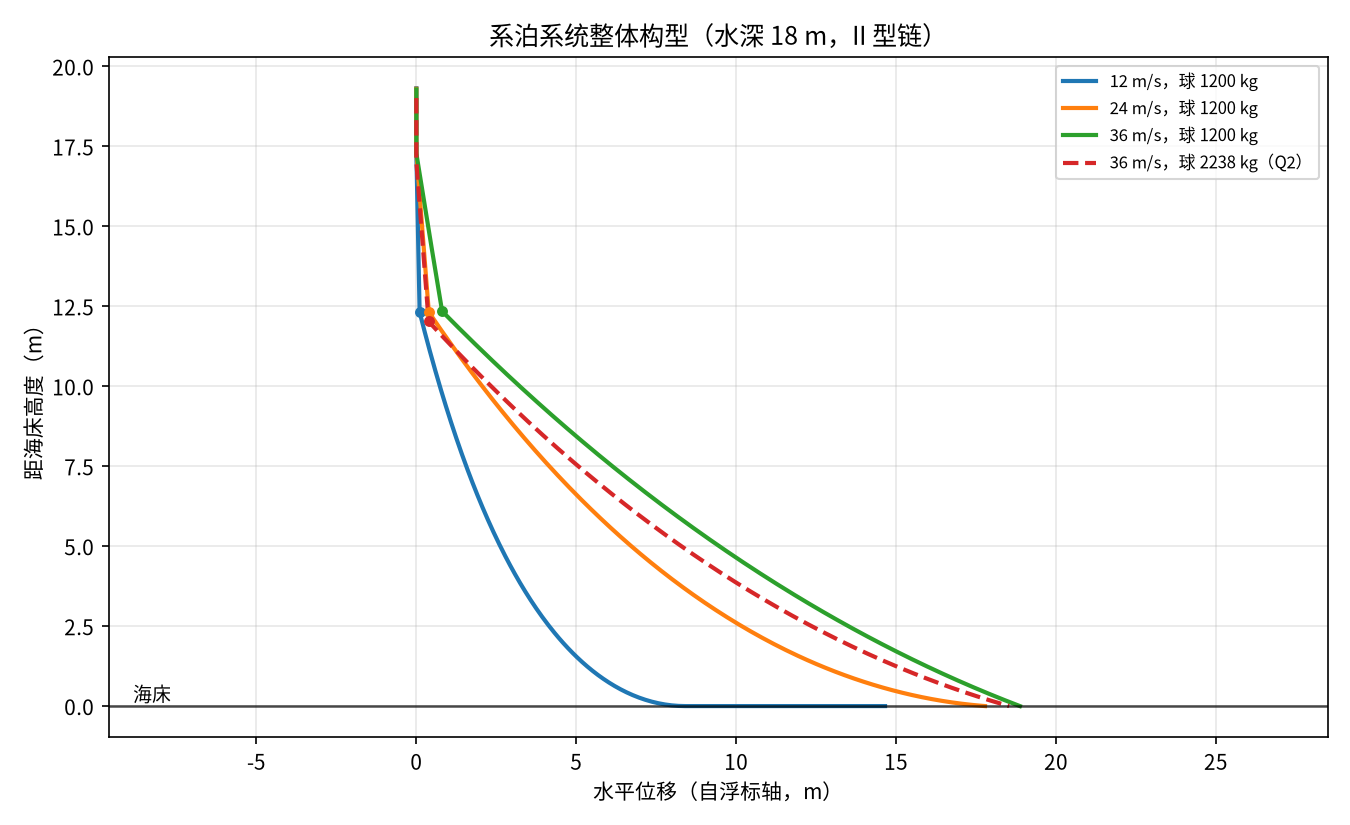
\includegraphics[width=0.92\textwidth]{fig_chain_shape.png}
\caption{系泊系统整体构型（水深 \SI{18}{m}，II 型链）}
\label{fig:shape}
\end{figure}

\begin{figure}[H]
\centering
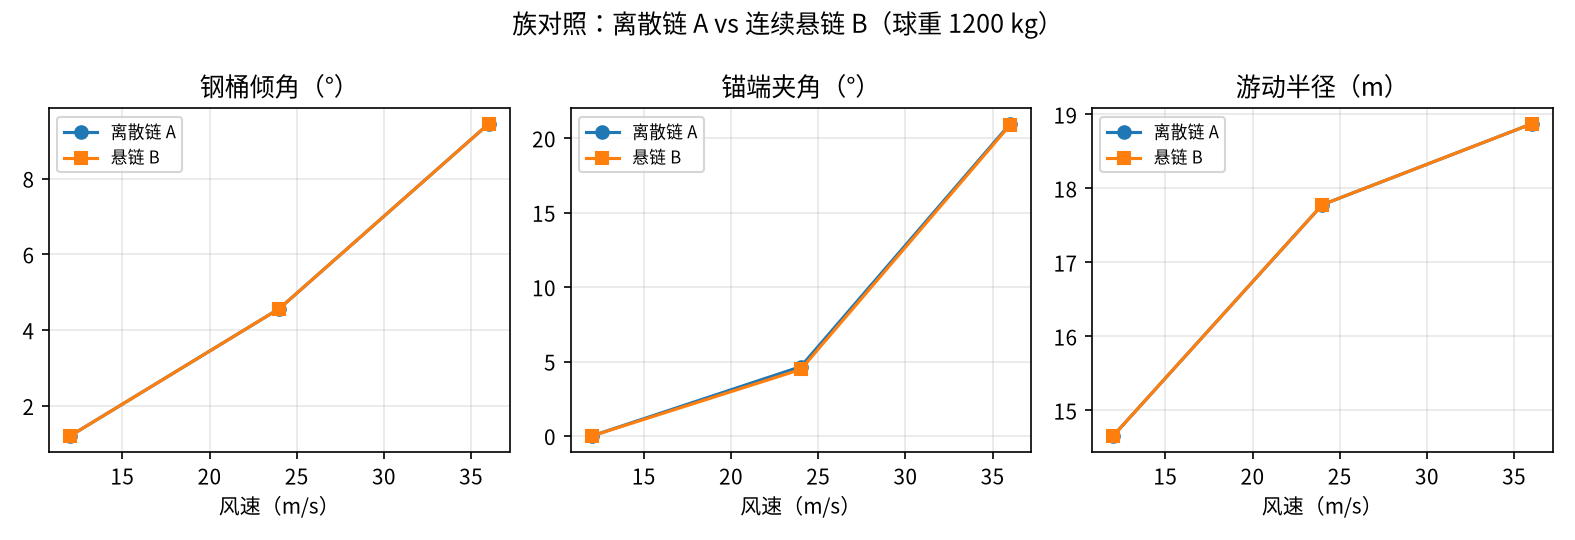
\includegraphics[width=0.98\textwidth]{fig_family_contrast.png}
\caption{族对照：离散链 A 与连续悬链 B（球重 \SI{1200}{kg}）}
\label{fig:family}
\end{figure}

\subsection{问题 2}
\label{sec:q2}

在 \SI{36}{m/s}、其余同问题 1 下，球重 \SI{1200}{kg} 不可行。粗网格 + 二分得最小可行球重 \textbf{\SI{2238}{kg}}：

\begin{table}[H]
\centering
\caption{问题 2 最小可行球重对应状态（Family A）}
\begin{tabular}{lc}
\toprule
量 & 数值 \\
\midrule
球重 & \SI{2238}{kg} \\
钢桶倾角 \(\theta\) & \(4.46^\circ\) \\
锚端夹角 \(\varphi\) & \(16.00^\circ\) \\
游动半径 \(R\) & \SI{18.53}{m} \\
吃水 \(d\) & \SI{0.990}{m} \\
钢管倾角 & \(4.37^\circ\)--\(4.42^\circ\) \\
\bottomrule
\end{tabular}
\end{table}

对照 B 的最小可行球重约 \SI{2220}{kg}（\(\Delta\approx 18\,\mathrm{kg}\)）。
球重--倾角曲线见图\ref{fig:ball}：\(\varphi\) 约束先于 \(\theta\) 成为紧约束。

\begin{figure}[H]
\centering
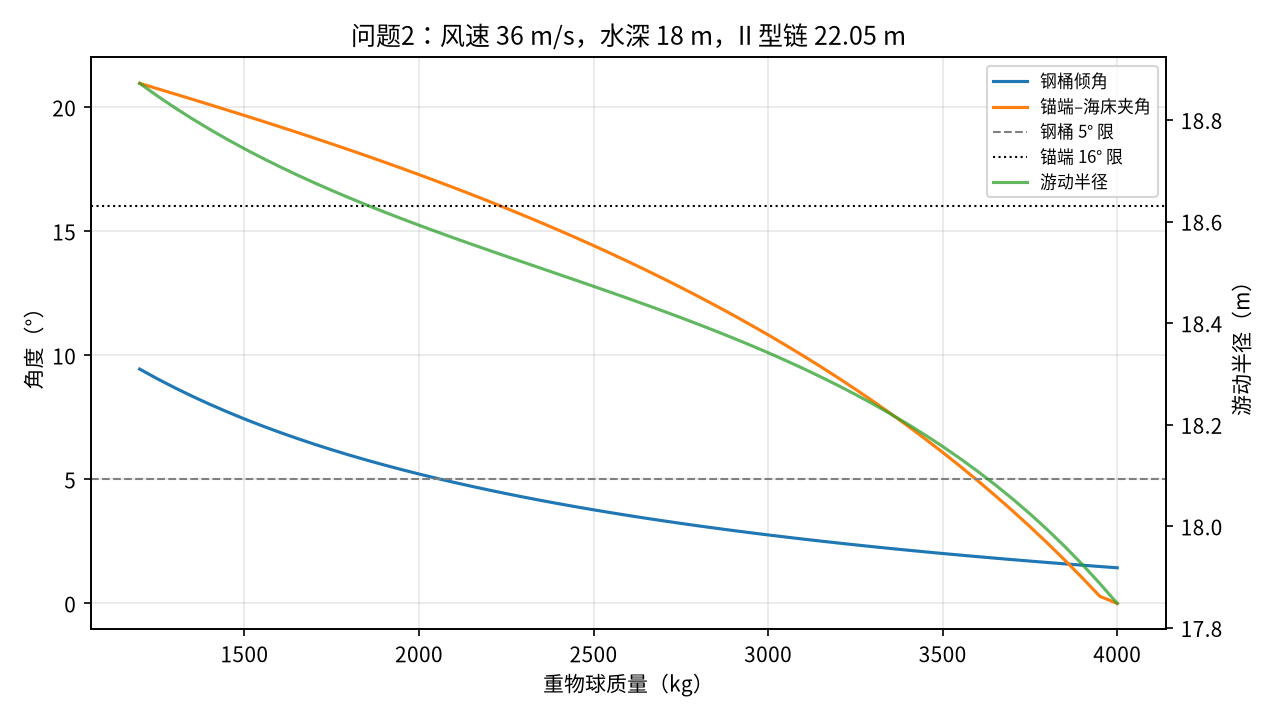
\includegraphics[width=0.92\textwidth]{fig_ball_sweep.png}
\caption{问题 2：球重扫描（风速 \SI{36}{m/s}）}
\label{fig:ball}
\end{figure}

\subsection{问题 3}
\label{sec:q3}

训练情景含（水深，\(v_w\)，\(v_c\)）角点与典型组合共 7 组；hold-out 5 组；稠密扫描 252 点仅评估。
候选均满足整数链节。网格上共 34 个硬约束全可行设计，其中 5 个同时满足软裕度；Pareto 前沿规模 26。

\noindent\textbf{推荐方案（软裕度 + 均衡效用）：IV 型锚链，长度 \SI{28.05}{m}（187 节），重物球 \SI{5000}{kg}。}

\begin{table}[H]
\centering
\caption{推荐方案在训练情景下的状态（Family A）}
\label{tab:q3}
\begin{tabular}{ccccccc}
\toprule
水深 & \(v_w\) & \(v_c\) & \(d\) & \(R\) & \(\theta_{\text{桶}}\) & \(\varphi_{\text{锚}}\) \\
(m) & (m/s) & (m/s) & (m) & (m) & (\(^\circ\)) & (\(^\circ\)) \\
\midrule
16 & 36 & 1.5 & 1.801 & 25.83 & 4.48 & 0.00 \\
18 & 36 & 1.5 & 1.816 & 25.00 & 4.44 & 0.00 \\
20 & 36 & 1.5 & 1.831 & 24.10 & 4.39 & 1.96 \\
18 & 24 & 1.0 & 1.781 & 23.43 & 2.02 & 0.00 \\
16 & 36 & 0   & 1.740 & 22.20 & 0.54 & 0.00 \\
20 & 36 & 0   & 1.760 & 18.73 & 0.49 & 0.00 \\
16 & 12 & 1.5 & 1.797 & 25.71 & 4.13 & 0.00 \\
\bottomrule
\end{tabular}
\end{table}

Hold-out 与稠密扫描：硬约束全部通过。
训练最劣：\(\theta\approx 4.48^\circ\)、\(\varphi\approx 1.96^\circ\)、最大吃水约 \SI{1.83}{m}。

机制：较大球重抬高吃水 \(\Rightarrow\) 干舷与 \(F_w\) 下降；重型链提高单位长度净重，利于趴链与控 \(\varphi\)。
分段流力使链顶 \(H\) 大于浮标端 \(H_0\)，比``全荷载集中到顶端''更符合传力路径。

\begin{table}[H]
\centering
\caption{问题 3 Pareto 备选}
\begin{tabular}{clrrr p{4.2cm}}
\toprule
取向 & 型号 & 链长(m) & 节数 & 球重(kg) & 说明 \\
\midrule
推荐（裕度均衡） & IV & 28.05 & 187 & 5000 & 软裕度全过 \\
更短游动 & V & 21.96 & 122 & 5000 & 平均 \(R\) 更小，吃水略高 \\
更低吃水 & IV & 30.00 & 200 & 4500 & 最大吃水约 \SI{1.70}{m}，\(\theta\) 裕度更紧 \\
\bottomrule
\end{tabular}
\end{table}

\begin{figure}[H]
\centering
\begin{subfigure}{0.98\textwidth}
\centering
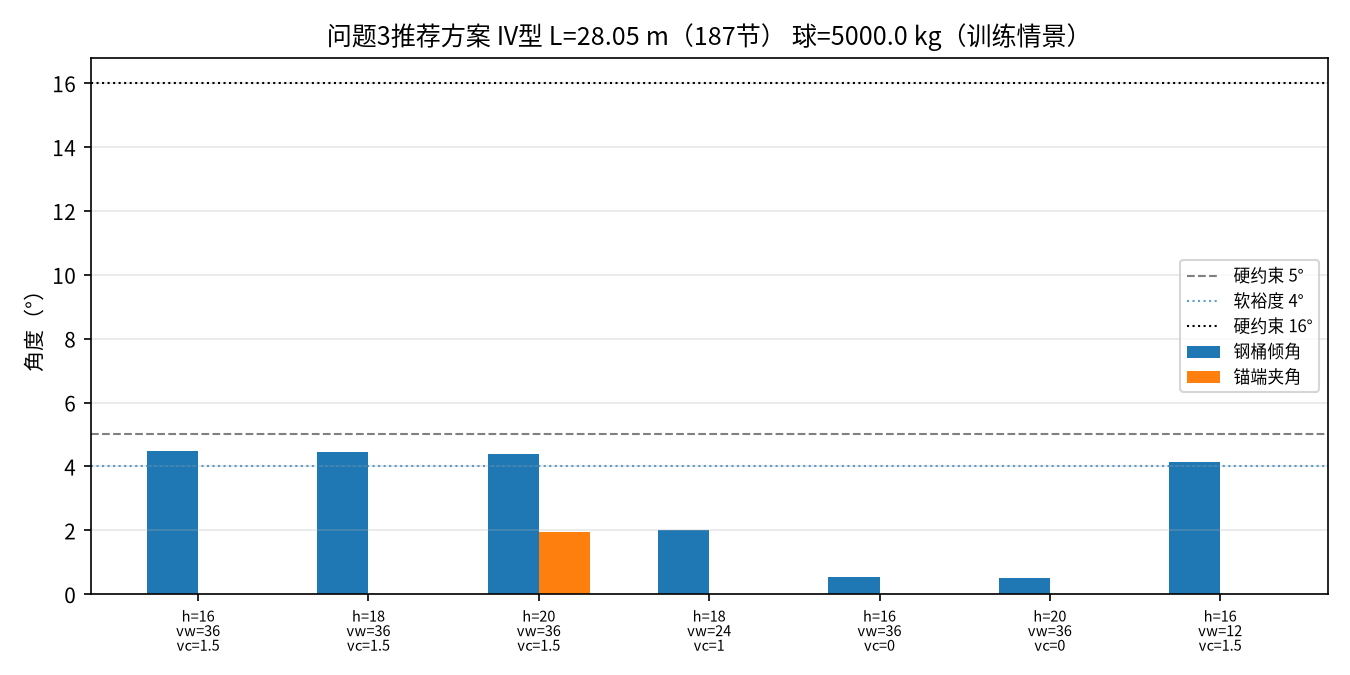
\includegraphics[width=0.92\textwidth]{fig_q3_scenarios.png}
\caption{推荐方案训练情景倾角}
\end{subfigure}

\vspace{0.8em}
\begin{subfigure}{0.98\textwidth}
\centering
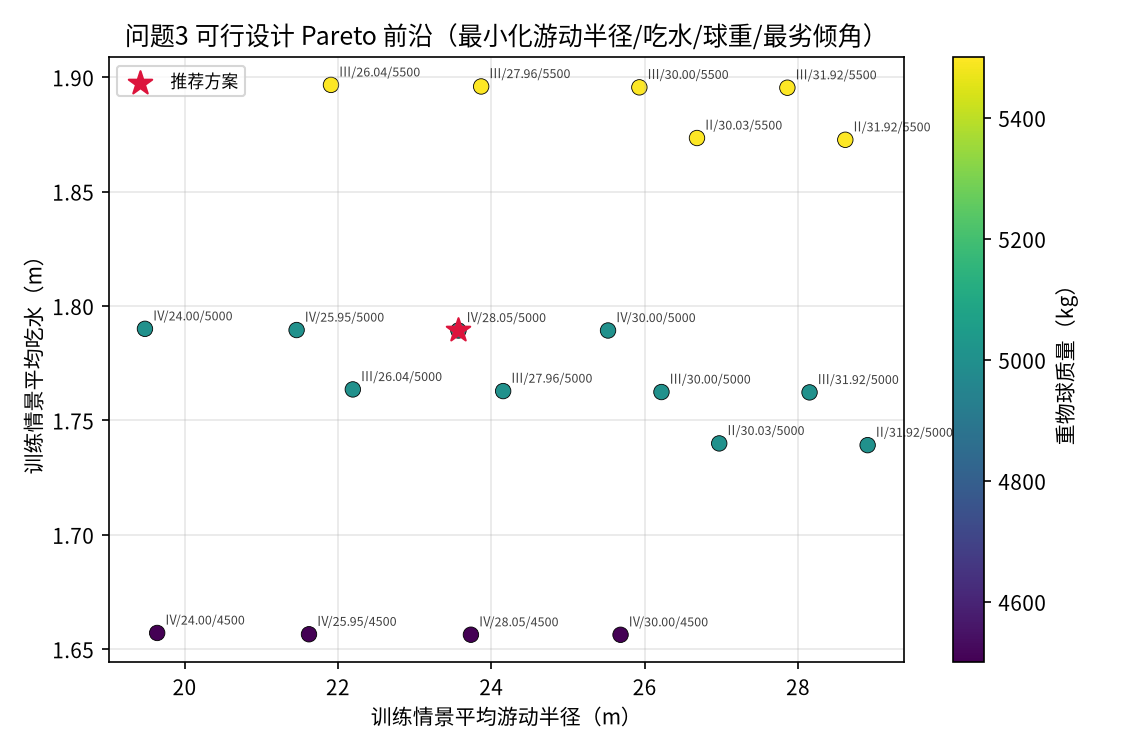
\includegraphics[width=0.86\textwidth]{fig_q3_pareto.png}
\caption{可行设计 Pareto 前沿}
\end{subfigure}
\caption{问题 3 结果图}
\label{fig:q3}
\end{figure}

\section{检验与敏感性}
\label{sec:check}

\begin{enumerate}[leftmargin=1.6em,itemsep=0.3em]
  \item \textbf{族对照：}A/B 主指标差 \(<\delta\)，离散误差非主矛盾。
  \item \textbf{球浮力消融（\SI{24}{m/s}）：}忽略球排水后 \(\theta_{\text{桶}}\) 由 \(4.57^\circ\to 3.85^\circ\)，并出现趴链，净重模块不可删。
  \item \textbf{密度敏感性：}\(\rho\in\{1020,1025,1030\}\) 时 \(\theta_{\text{桶}}\in[4.55^\circ,4.58^\circ]\)，\(\varphi\in[4.54^\circ,4.78^\circ]\)，变化 \(<\delta\)。
  \item \textbf{整数链节：}名义 \SI{22.05}{m} 对 V 型不可整除（\(22.05/0.18=122.5\)），搜索中已剔除。
  \item \textbf{分段 \(H\)：}有流情景下链顶水平张力高于浮标端，避免上部杆被下游流力错误加载。
  \item \textbf{反事实：}``加重球必定增大游动半径''与扫描不符——可行域内 \(R\) 随球重缓变，约束改善由 \(\theta,\varphi\) 主导。
  \item \textbf{泄漏控制：}问题 3 选型仅用训练情景；hold-out 与稠密扫描未参与选型。
\end{enumerate}

\section{优缺点与讨论}

\textbf{优点（有证据）：}基线可复现；A/B 交叉验证；分段流力与整数链节贴近物理/制造；
问题 2/3 约束可检查；Pareto 与软裕度避免单一字典序冒充``最优''。

\textbf{缺点 / 中等风险：}
\begin{itemize}[leftmargin=1.6em,itemsep=0.2em]
  \item 静力、无浪；实际海域可能偏危险侧。
  \item 风/流投影与均匀流、共面简化。
  \item 问题 3 仍为离散网格推荐；效用权重可影响折中点（故同时报告备选）。
  \item 推荐方案吃水仍偏高（约 \SI{1.8}{m}），对密度/附着等扰动敏感。
\end{itemize}

致命项在静力题面内未检出；外推有浪条件须重新建模。

\section{改进方向}

\begin{enumerate}[leftmargin=1.6em,itemsep=0.25em]
  \item 引入规则波或谱浪下的准静力/时域张力包络。
  \item 流剖面与三维风向不一致时的矢量合成。
  \item 在可行域内对（型号，链长，球重）做更细网格或连续松弛的多目标搜索。
  \item 锚抓力曲线替代单纯 \(\varphi\le 16^\circ\) 代理。
  \item 将钢管--钢桶--链条的流力系数由题面公式校准为分项 \(C_d\)。
\end{enumerate}

\section{结论}

在给定静力假设与 Freeze \texttt{2016A-mooring-F2} 证据下：
\begin{enumerate}[leftmargin=1.8em,itemsep=0.35em]
  \item 问题 1 给出 \(12/24\,\mathrm{m/s}\) 全套几何与倾角，\SI{24}{m/s} 仍满足工作约束；
  \item 问题 2 在 \SI{36}{m/s} 需将球重提至 \textbf{\SI{2238}{kg}} 方同时满足 \(\theta\le 5^\circ\) 与 \(\varphi\le 16^\circ\)；
  \item 问题 3 在整数链节与分段流力模型下，推荐 \textbf{IV 型、\SI{28.05}{m}（187 节）、球 \SI{5000}{kg}}，
        训练/hold-out/稠密扫描硬约束通过，并给出更短游动与更低吃水的 Pareto 备选；
        适用性限于本题静力与投影假设。
\end{enumerate}

\appendix
\section{结果文件索引}

\begin{itemize}[leftmargin=1.6em]
  \item \texttt{results/metrics.json}：全量数值
  \item \texttt{results/results\_tables.xlsx}：多工作表结果表（便于查阅）
  \item \texttt{results/fig\_*.png}：构型、扫描、族对照、情景与 Pareto 图
  \item \texttt{code/mooring\_solve.py}、\texttt{code/export\_xlsx.py}、\texttt{code/make\_figures.py}
\end{itemize}

\section{主要符号表}

\begin{table}[H]
\centering
\caption{主要符号}
\begin{tabular}{cl}
\toprule
符号 & 含义 \\
\midrule
\(d\) & 浮标吃水 \\
\(H_u,H_{\ell}\) & 杆段上/下端水平张力 \\
\(F_c\) & 构件水流力 \\
\(\theta\) & 与竖直线夹角 \\
\(\varphi\) & 锚端切线与海床夹角 \\
\(R\) & 游动半径（锚到浮标轴水平距） \\
\(w\) & 锚链单位长度水中净重 \\
\(N\) & 锚链节数 \\
\bottomrule
\end{tabular}
\end{table}

\end{document}
